%\title{Truncated Exponential Sampling}
%\author{Emanuel Casiano-Diaz}
%\date{January 19, 2022.}


%Formatting Packages
\documentclass[12pt, two sided]{article}
\usepackage[utf8]{inputenc}
%\usepackage[letter,top=1.1in,bottom=1.1in,left=1.6in,right=1.1in]{geometry}
\usepackage[letterpaper,margin=1in]{geometry}

\usepackage{graphicx}
\usepackage{subfig}
\usepackage{float}

%Math Packages
\usepackage{amsmath}
\usepackage{amssymb}
\usepackage{bm}
\DeclareMathOperator{\Tr}{Tr}

%Physics Package
\usepackage{physics}

%Allow accentuation marks
\usepackage[utf8]{inputenc}
\usepackage[T1]{fontenc}

%Image packages
\usepackage{graphicx}
\graphicspath{ {Images/} }

%Enumerating lists
\usepackage{enumerate}% http://ctan.org/pkg/enumerate

%Adjust depth of subsections
\setcounter{secnumdepth}{3}

%Adjust depth of table of contents
\setcounter{tocdepth}{3}

%References Packages
%\usepackage{biblatex}
%\addbibresource{references.bib}
\usepackage[bookmarks=true]{hyperref}
\hypersetup{
    hidelinks=true,
    linkcolor=blue,
    filecolor=magenta,      
    urlcolor=cyan,
}

%Commands and packages imported from particle entanglement paper
\usepackage{amsmath}
\usepackage{xcolor}
\usepackage{graphicx}
\usepackage{amssymb}

\newcommand{\eket}[1]{\bigl \vert #1 \bigr \rangle}
\newcommand{\R}{\boldsymbol{R}}
\newcommand{\Rt}{\tilde{\R}}
\newcommand{\ebra}[1]{\bigl \langle #1 \bigr \vert}
\newcommand{\eexp}[1]{\bigl \langle #1 \bigr \rangle}
\newcommand{\figref}[1]{Fig.~\ref{#1}}
\renewcommand{\vec}[1]{\boldsymbol{#1}}
\newcommand{\ren}{R\'{e}nyi~}
\newcommand{\rnote}[1]{{\it \textcolor{red}{#1} }}
\newcommand{\Eqref}[1]{Eq.~\eqref{#1}}

%Copied from paper
\usepackage{color}
\usepackage{graphicx}
\usepackage[color=green!60]{todonotes}
\usepackage{physics}
\usepackage{amsthm}
\usepackage{amsmath}
\usepackage{amssymb}
\usepackage{enumerate}
\usepackage{placeins}
\usepackage{booktabs}
\usepackage{dsfont}

%For reference formatting
\usepackage[numbers,sort&compress]{natbib}
\bibliographystyle{nsf_new_url}

\setlength{\footskip}{22pt}

 %Line spacing
\usepackage{setspace}
\doublespace

% --------- Begin Document -------- %
\begin{document}

%----- Introduction -------%


\section{Introduction}

Restricted Boltzmann Machines (RBMs) are neural networks that can reproduce a probability distribution, given a set of training samples. They have the architectural peculiarity of being composed of one visible (input) layer and one hidden layer. As opposed to general Boltzmann Machines, they are restricted in the sense that the units, or neurons, are not connected to other units in the same layer, only ones in the other layer. The values themselves of the units are binary (i.e, 0 or 1).

\begin{figure}[h!]
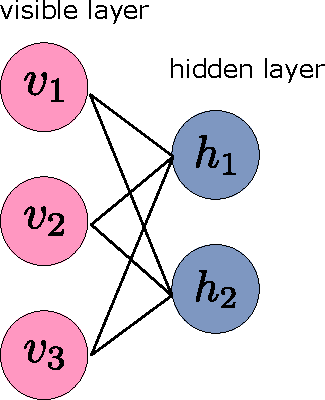
\includegraphics[width=8cm]{Figures/rbm.pdf}
\caption{Example RBM with visible layer $\mathbf{v}$ consisting of $D=3$ units and hidden layer consisting of $n_h=2$ units.}
\end{figure} 

%-----------------------------   Theory ----------------------------------------------% 

\section{Theory}

Consider an RBM with a visible layer $\mathbf{v}$ of length $D$ and hidden layer $\mathbf{h}$ of length $n_h$, where each component of $\mathbf{v}$ and $\mathbf{h}$ can be either 0 or 1 and let the parameters of this network be $\lambda=\lbrace \mathbf{a,b,w} \rbrace$. The probability of a configuration consisting of visible layer $\mathbf{v}$ and hidden layer $\mathbf{h}$, with parameters $\lambda$, is given by the joint Boltzmann distribution:

\begin{equation}
P(\mathbf{v},\mathbf{h}) = \frac{e^{-E(\mathbf{v},\mathbf{h})}}{\mathcal{Z}_{\lambda}} 
\end{equation}

where the partition function is: 

\begin{equation}
\mathcal{Z}_{\lambda} = \sum_{\mathbf{v},\mathbf{h}} e^{-E(\mathbf{v},\mathbf{h})}
\end{equation}

and the "energy" is:

\begin{equation}
E(\mathbf{v},\mathbf{h}) = -\sum_{i=1}^D a_i v_i - \sum_{j=1}^{n_h} b_i h_i - \sum_{i,j} v_i w_{ij} h_j
\end{equation}

The marginalized probability of a visible vector can be obtained by summing out the hidden vector dependence:

\begin{equation}
P(\mathbf{v}) = \frac{1}{{\mathcal{Z}_{\lambda}}} \sum_{\mathbf{h}} e^{-E(\mathbf{v,h})}
\end{equation}

and likewise for the marginal probability of a hidden vector:

\begin{equation}
P(\mathbf{h}) = \frac{1}{{\mathcal{Z}_{\lambda}}} \sum_{\mathbf{v}} e^{-E(\mathbf{v,h})}
\end{equation}

The conditional probability of a visible vector given a hidden vector is:

\begin{equation}
P_{\lambda}(\mathbf{v} \vert \mathbf{h}) = \prod_{i=1}^{D} P_{\lambda}(v_i \vert \mathbf{h})
\end{equation}

where the factorization of probabilities is due to the fact the input unit activations $v_i$ are mutually independent, since there are no connections between units in the same layer. Similarly, the probability of a hidden vector given an input is:

\begin{equation}
P_{\lambda}(\mathbf{h} \vert \mathbf{v}) = \prod_{j=1}^{n_h} P_{\lambda}(h_j \vert \mathbf{v})
\end{equation}

The activation probabilities of each unit are given by:

\begin{equation}
P_{\lambda}(h_j \vert \mathbf{v}) = 
\begin{cases}
\sigma(z_j) &\, h_j = 1\\
1 - \sigma(z_j) &\, h_j = 0
\end{cases}
\end{equation}

where $\sigma(z)$ is the logistic sigmoid function:

\begin{equation}
\sigma(z_j) = \frac{1}{1+e^{-z_j}}
\end{equation}

and $z_j$ is the weighted sum of inputs:

\begin{equation}
z_j = b_j + \sum_{i=1}^{D} v_i w_{ij}
\end{equation}

The activation probabilities of input units are obtained similarly, replacing the weighted sum of inputs with:

\begin{equation}
z_i = a_i + \sum_{j=1}^{n_h} h_j w_{ij}
\end{equation}

Using these probabilities, a Markov chain can be produced that generates hidden vectors from visible ones, and from the generated hidden vector, a new visible one:

\[\bf v \to h^\prime \to v^\prime \to h^{\prime\prime} \to v^{\prime\prime} \to h^{\prime\prime\prime} \to \dots\]

At the end of the random walk, a model for the probability distribution of input vectors is obtained.

%-----------------------------   Training ----------------------------------------------% 

\section{Training}

Typically, RBMs are trained using the method of contrastive divergence (CD), which performs Gibbs sampling, and inside a gradient descent (GD) procedure, which updates the network weights.

Unbiased samples are obtained via alternating Gibbs sampling using the unit activation probabilities derived in the previous section.

The cost function to be used is:

\begin{equation}
C = -\sum_{\mathbf{v}} P(\mathbf{v}) \ln P_{\lambda}(\mathbf{v})
\end{equation}

which is known as the Kullback-Leibler divergence, without the constant term. (Alternatively, it is the difference between two Kullback-Leibler divergence functions)

For network parameters $\lambda = \lbrace \mathbf{a}, \mathbf{b}, \mathbf{w} \rbrace$, the gradients for GD are:

\begin{equation}
\delta_a = \frac{\partial C}{\partial a_i} = -\langle v_i \rangle + \langle v_i^{\prime}\rangle
\end{equation}

\begin{equation}
\delta_b = \frac{\partial C}{\partial b_j} = -\langle h_j \rangle + \langle h_j^{\prime}\rangle
\end{equation}

\begin{equation}
\delta_w = \frac{\partial C}{\partial w_{ij}} = -\langle v_i h_j \rangle + \langle v_i^{\prime} h_j^{\prime}\rangle
\end{equation}

The averages that show up in the gradients are computed by taking the average of the unit over sample in the batch, or mini-batch:

\begin{equation}
\langle v_i \rangle = \frac{1}{N_{\rm{mini}}} \sum_{n=1}^{N_{\rm{mini}}} v_i^{(n)}
\end{equation}

\begin{equation}
\langle h_j \rangle = \frac{1}{N_{\rm{mini}}} \sum_{n=1}^{N_{\rm{mini}}} h_j^{(n)}
\end{equation}

\begin{equation}
\langle v_i h_j \rangle = \frac{1}{N_{\rm{mini}}} \sum_{n=1}^{N_{\rm{mini}}} v_i^{(n)} h_j^{(n)}
\end{equation}

To track the training progress, the cost function needs to be computed for the various iterations of network parameters. Computing it though, will not be tractable due to the exponentially large size of the configuration space of hidden-visible vector pairs:

\begin{align}
C &= -\sum_{\mathbf{v}} P_{\lambda}(\mathbf{v}) \ln P_{\lambda}(\mathbf{v}) \\
&\approx -\frac{1}{N} \sum_{n=1}^{N} \ln P_{\lambda}(\mathbf{v}^{(n)}) \\
&= -\frac{1}{N} \sum_{n=1}^{N} [\sum_{\mathbf{h}} \ln P_{\lambda}(\mathbf{v}^{(n)},\mathbf{h})] \\
C &= -\frac{1}{N} \sum_{n=1}^{N} F(\mathbf{v}^{(n)}) + \ln \mathcal{Z}_{\lambda}
\end{align}

where the "free energy" $F(\mathbf{v}^{(n)})$ is defined such that:

\begin{equation}
e^{-F(\mathbf{v})} = \sum_{\mathbf{h}} e^{-E(\mathbf{v,h})}
\end{equation}

which is exponentially hard to compute.

There are three alternative approaches to keep track of the training progress:

\textbf{Approach 1: Track squared error between data and reconstructions}

\begin{equation}
C_1 = \frac{1}{N} \sum_{n=1}^{N} \| \boldsymbol{v}^{(n)} - \boldsymbol{v}^{(n)\prime} \|^2
\end{equation}

\textbf{Approach 2: Track categorical cross-entropy of visible layer's binary units.}

\begin{equation}
C_2 = - \frac{1}{N} \sum_{n=1}^{N} \left\{ \sum_{i=1}^{D} v_i  \log \sigma(\tilde{z}_i) + (1-v_i) \log \left[1-\sigma(\tilde{z}_i) \right] \right \}
\end{equation}

where $ \tilde{z}_i = a_i + \sum_{j=1}^{n_h} w_{ij} h_j\ $ .

\textbf{Approach 3: Compare current free-energy to free-energy of validation data. The hope is that these should be approximately equal.}

\begin{equation}
C_3 = \left\lvert \frac{1}{N_{\rm val}}  \sum_{n=1}^{N_{\rm val}} F(\boldsymbol{v}_{\rm val}^{(n)}) - \frac{1}{N} \sum_{n=1}^{N} F(\boldsymbol{v}^{(n)}) \right \rvert
\end{equation}

%-----------------------------   Results ----------------------------------------------% 

\section{Results}

\textbf{Example visible vectors for training}
\begin{figure}[h!]
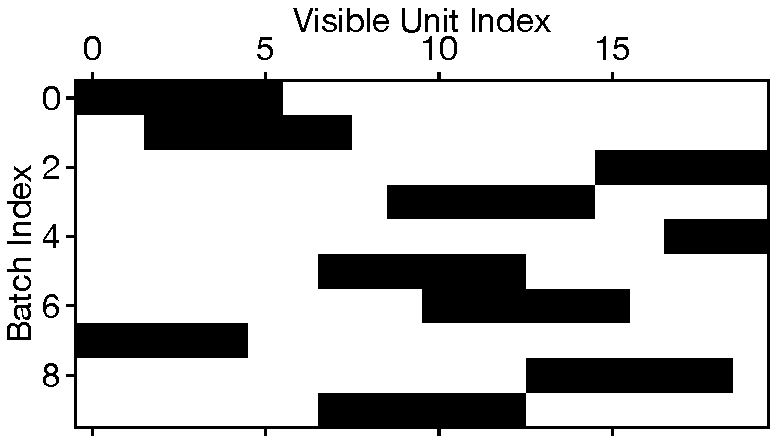
\includegraphics[width=8cm]{Figures/training_visible_vectors.pdf}
\end{figure} 

\textbf{Comparison of cost function alternative approaches}
\begin{figure}[h!]
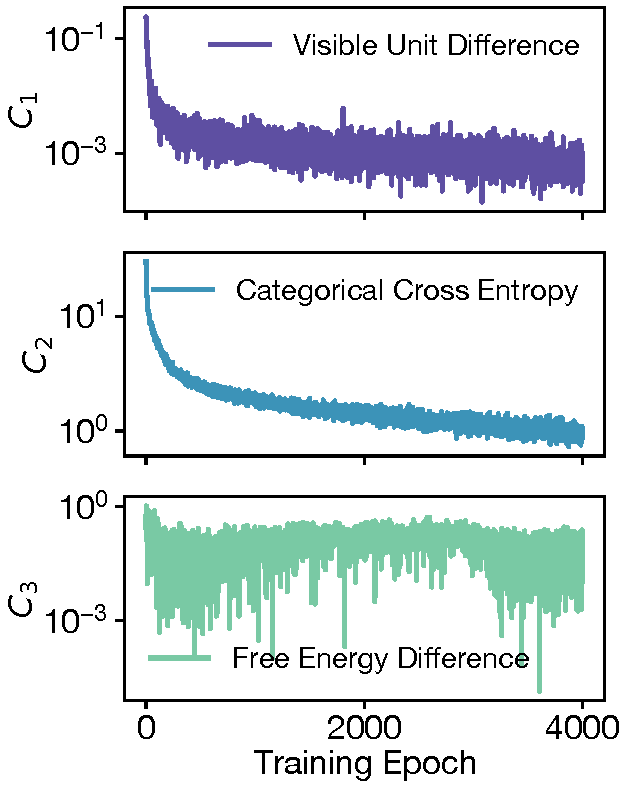
\includegraphics[width=8cm]{Figures/cost_function_approaches.pdf}
\end{figure} 

\textbf{Sampled visible vectors}
\begin{figure}[h!]
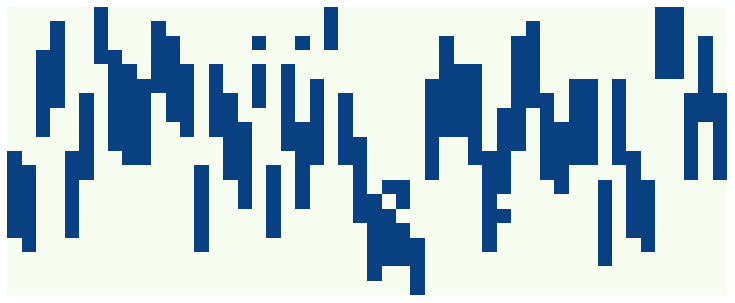
\includegraphics[width=8cm]{Figures/sampled_visible_vectors.pdf}
\end{figure} 

\section{Ising model}

\begin{figure}[h!]
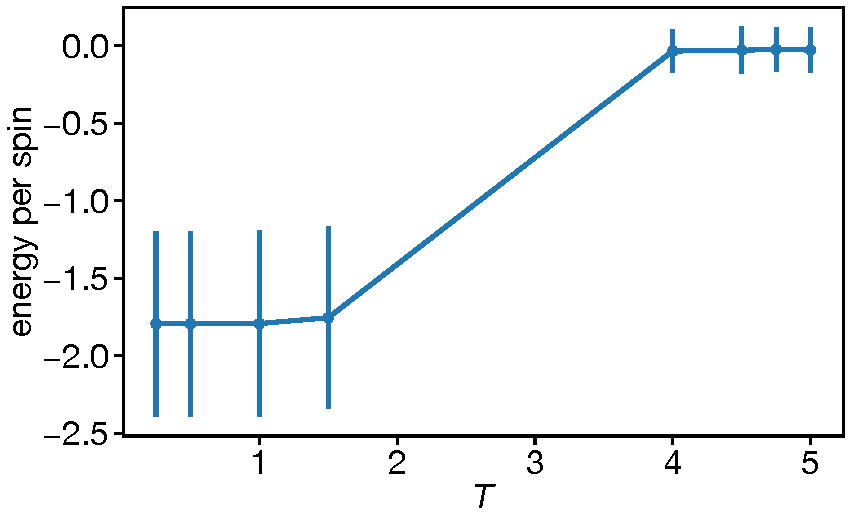
\includegraphics[width=8cm]{Figures/rbm_e.pdf}
\caption{Energy per spin on a $10\times10$ lattice.}
\end{figure} 

\begin{figure}[h!]
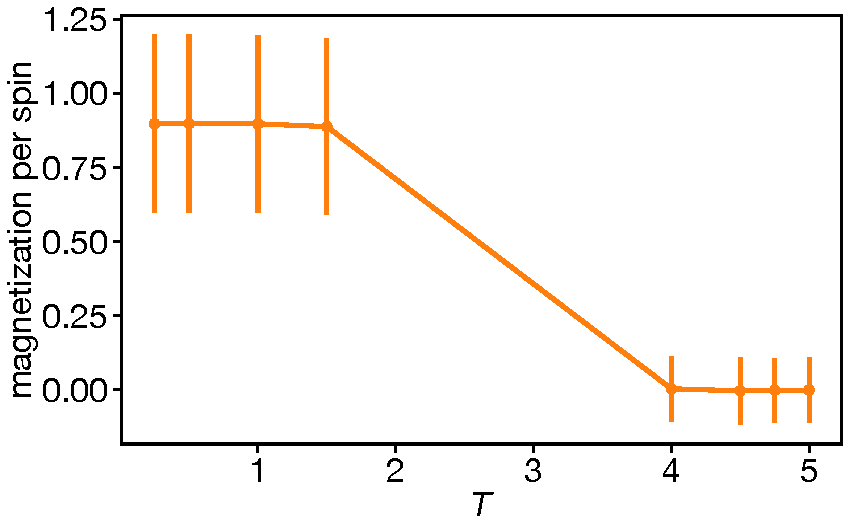
\includegraphics[width=8cm]{Figures/rbm_m.pdf}
\caption{Magnetization per spin on a $10\times10$ lattice.}
\end{figure} 

% ------------------------------------------------------ end ---------------------------------- %

% References (ugly version)

\section{References}

\begin{itemize}
\item Adrian's Machine Learning Lecture notes \\
\item \url{https://en.wikipedia.org/wiki/Restricted_Boltzmann_machine} \\
\item \url{http://www.cs.toronto.edu/~hinton/absps/guideTR.pdf} \\
\item \url{https://www.nature.com/articles/s41567-019-0545-1}
\end{itemize}

% References
\phantomsection 
\addcontentsline{toc}{chapter}{References} 
%\bibliographystyle{apalike} %acm, ieetr, apalike...
 %\section*{Referencess
 \singlespacing
\bibliography{references}

\doublespacing

\end{document}
